\section{Annealed Stein variational gradient descent}\label{sec:asvgd} 




\captionsetup[subfigure]{labelformat=empty}
\begin{figure}[t!]
    \centering 
\begin{subfigure}[b]{.48\textwidth} 
    \scalebox{1}{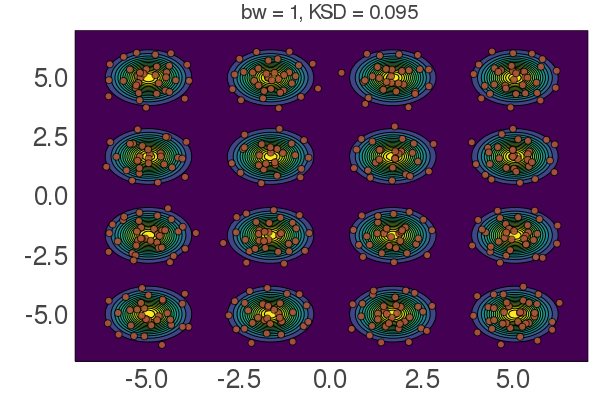
\includegraphics[width=\textwidth]{figures/bw1.png}}
    \caption{(a)\label{fig:bw1}}
\end{subfigure}
\hfill
\centering
\begin{subfigure}[b]{0.48\textwidth}
    \scalebox{1}{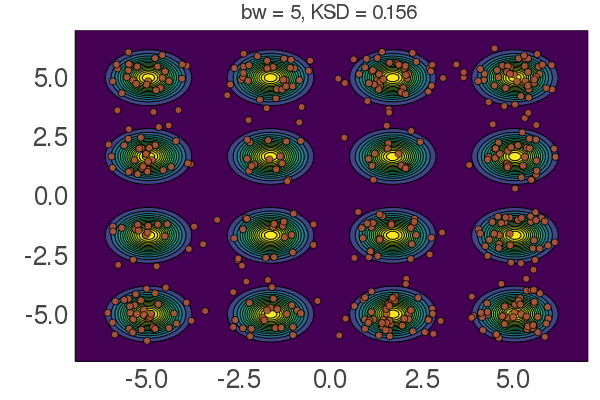
\includegraphics[width=\textwidth]{figures/bw5.png}}
    \caption{(b)\label{fig:bw5}}
\end{subfigure}
\hfill
\centering
\begin{subfigure}[b]{0.48\textwidth}
    \scalebox{1}{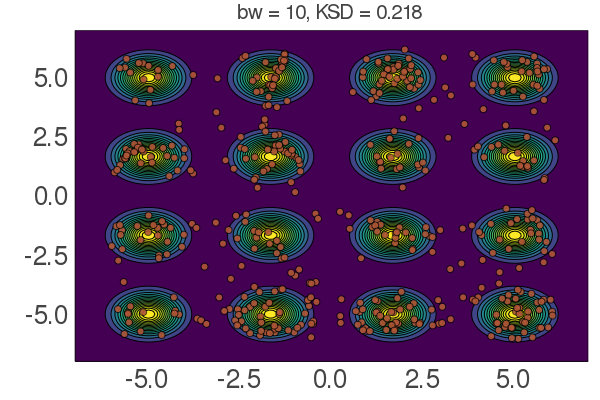
\includegraphics[width=\textwidth]{figures/bw10.png}}
    \caption{(c)\label{fig:bw10}}
\end{subfigure}
\hfill
\centering
\begin{subfigure}[b]{0.48\textwidth}
    \scalebox{1}{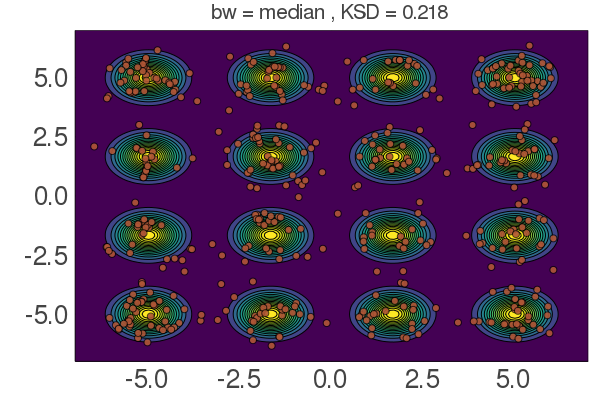
\includegraphics[width=\textwidth]{figures/bwmed.png}}
    \caption{(d)\label{fig:bwmed}}
\end{subfigure}

\caption{Comparison of A-SVGD on the synthetic Gaussian mixture with 16 components across different bandwidth. }
\label{fig:BW}
\end{figure}








\captionsetup[subfigure]{labelformat=empty}
\begin{figure}[t!]
    \centering 
\begin{subfigure}[b]{.48\textwidth} 
    \scalebox{1}{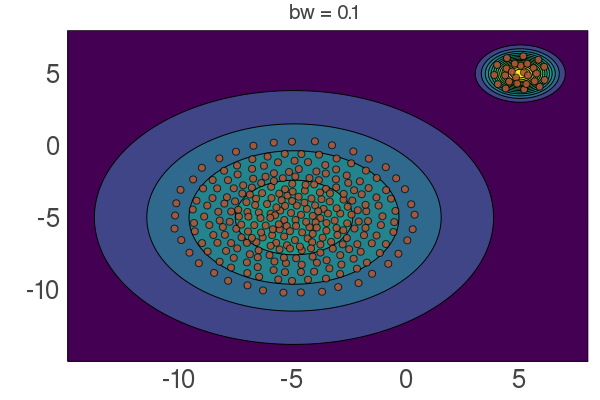
\includegraphics[width=\textwidth]{figures/bwsmall.png}}
    \caption{(a)\label{fig:bwsmall}}
\end{subfigure}
\hfill
\centering
\begin{subfigure}[b]{0.48\textwidth}
    \scalebox{1}{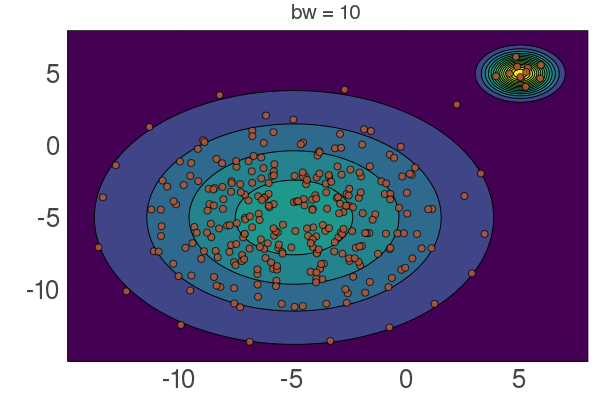
\includegraphics[width=\textwidth]{figures/bwlarge.png}}
    \caption{(b)\label{fig:bwlarge}}
\end{subfigure}
\hfill
\centering
\begin{subfigure}[b]{0.48\textwidth}
    \scalebox{1}{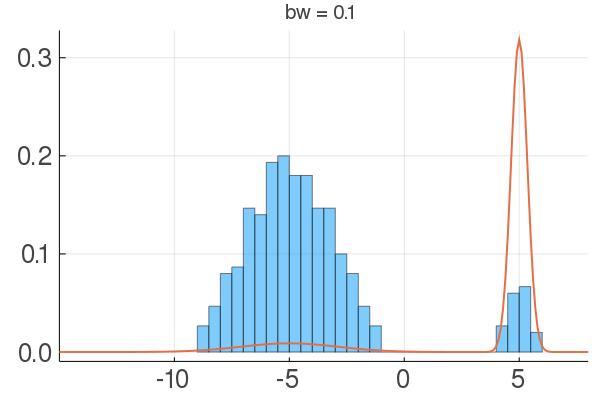
\includegraphics[width=\textwidth]{figures/slice_small.png}}
    \caption{(c)\label{fig:slice_small}}
\end{subfigure}
\hfill
\centering
\begin{subfigure}[b]{0.48\textwidth}
    \scalebox{1}{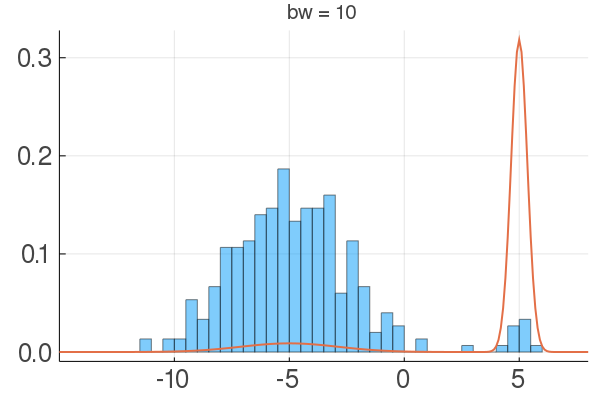
\includegraphics[width=\textwidth]{figures/slice_large.png}}
    \caption{(d)\label{fig:slice_large}}
\end{subfigure}


\caption{Comparison of A-SVGD on a 2-component Gaussian mixture with different bandwidth. \cref{fig:bwsmall,fig:bwlarge} show scatter plots of particles at the last iteration. \cref{fig:slice_small,fig:slice_large} show histograms of the particles by projecting the locations to the line $y = x$, where the orange curve denotes the density of Gaussian mixture along the slice $y = x$.}
\label{fig:differentBW}
\end{figure}


\begin{figure}[t!]
    
\end{figure}


\captionsetup[subfigure]{labelformat=empty}
\begin{figure}[t!]
    \centering 
\begin{subfigure}[b]{.48\textwidth} 
    \scalebox{1}{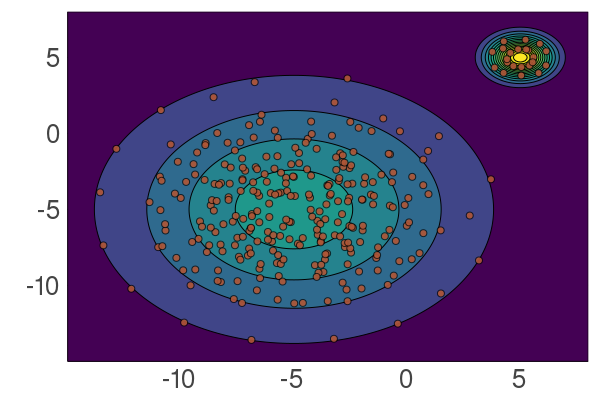
\includegraphics[width=\textwidth]{figures/bwlocal.png}}
    \caption{(a) \label{fig:bwlocal}}
\end{subfigure}
\hfill
\centering
\begin{subfigure}[b]{0.48\textwidth}
    \scalebox{1}{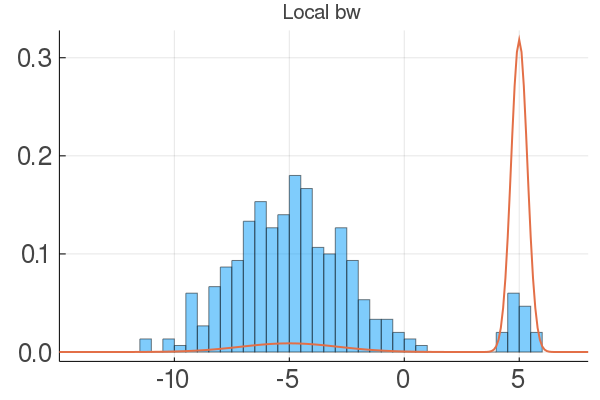
\includegraphics[width=\textwidth]{figures/slice_local.png}}
    \caption{(b)\label{fig:slicelocal}}
\end{subfigure}

\caption{A-SVGD with adaptive local bandwidth on a 2-component Gaussian mixture.}
\label{fig:localbw}
\end{figure}


\captionsetup[subfigure]{labelformat=empty}
\begin{figure}[t!]
    \centering 
\begin{subfigure}[b]{.48\textwidth} 
    \scalebox{1}{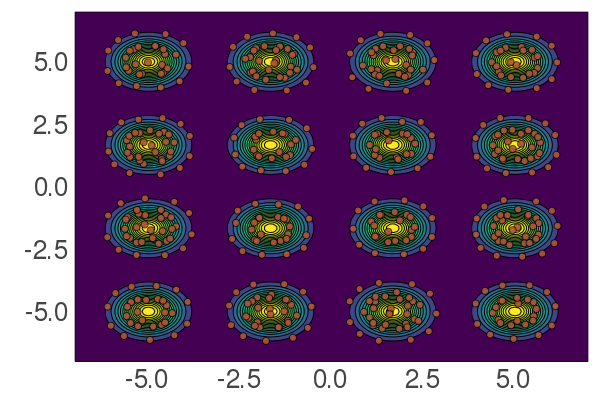
\includegraphics[width=\textwidth]{figures/grid_local.png}}
    \caption{(a) $\{x_i^{(0)}\}_{i = 1}^{500} \distiid \distNorm(0\ind, 0.25I)$  \label{fig:bwlocal}}
\end{subfigure}
\hfill
\centering
\begin{subfigure}[b]{0.48\textwidth}
    \scalebox{1}{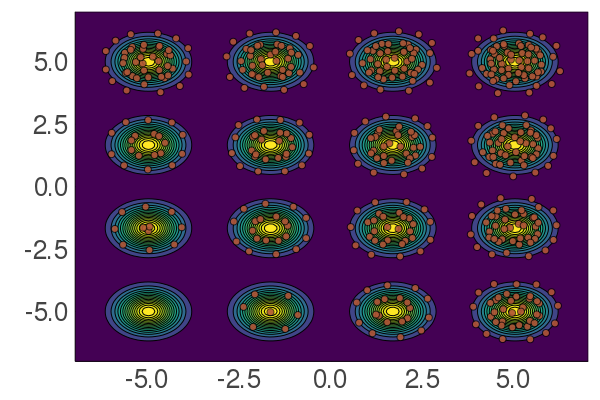
\includegraphics[width=\textwidth]{figures/grid_local10.png}}
    \caption{(b) $\{x_i^{(0)}\}_{i = 1}^{500} \distiid \distNorm(10\ind, 0.25I)$ \label{fig:slicelocal}}
\end{subfigure}

\caption{A-SVGD with adaptive local bandwidth on a $4 \times 4$ Gaussian mixture.}
\label{fig:gridlocal}
\end{figure}



In this section, we provide a brief introduction of the annealed SVGD (A-SVGD), which is developed to address the mixing issue \citep{d2021annealed}, and use a few synthetic examples to identify a key limitation of the current work. The design of the synthetic example aims to  understand the influence of the kernel bandwidth on the behaviour of SVGD or A-SVGD and help us to build the intuition of picking a proper value. All the experiments performed in this report use the RMSprop update rule \cref{eq:rms}. We run both SVGD and A-SVGD with standard RBF kernel for $1000$ iterations under a constant learning rate $\gamma_k = 0.1$. 



We start with the development of A-SVGD. Considering the updates \cref{eq:svgd}, the optimal descent direction $ \hat{\phi}^{\star}(x)$ for the particle $x$ includes two parts: the driving force that moves the particle to a high density region of $p(x)$, and a repulsion that prevents the particles collapsing together. The specific derivation is as follows,
\[
    \hat{\phi}_k^{\star}(x)=\frac{1}{n} \sum_{j=1}^{n}\left[\underbrace{\kappa\left(x_{j}^{(k)}, x\right) \nabla \log p\left(x_{j}^{(k)}\right)}_{\text {driving force }}+\underbrace{\nabla_{x_{j}^{(k)}} \kappa\left(x_{j}^{(k)}, x\right)}_{\text {repulsion }}\right].
\]
When mode collapse occurs, particles produced by SVGD are trapped at some region and fail to explore the full support of $p(x)$. This often happens when the driving force dominates the repulsion. An intuitive solution is to boost the repulsion or scale down the driving force to enable a wider spread of the particles. 
\citet{d2021annealed} follows this intuition and modify the descent direction by introducing an annealing term $\alpha(k) \in [0, 1]$:
\[\label{eq:asvgd}
    \hat{\phi}_{\alpha_k}\left(x\right) = \frac{1}{n} \sum_{j=1}^{n}\left[ \alpha(k)\kappa\left(x_{j}^{(k)}, x\right) \nabla \log p\left(x_{j}^{(k)}\right)+ \nabla_{x_{j}^{(k)}} \kappa\left(x_{j}^{(k)}, x\right)\right].
\]
In particular, the authors suggest using a cyclical annealing schedule, i.e., 
\[
    \alpha(k)=\left(\frac{\bmod (k, K / C)}{K / C}\right)^{p},
\]
where $K$ is the total number of iterations, $C$ is the number of cycles, and $p > 0$ is an exponent factor that controls the speed of the transition between two phases. As demonstrated in \cref{fig:acsched}, smaller $p$ corresponds to a shorter period of the exploratory phase.  In all our experiments using A-SVGD, we set $ p = 1$ and $C = 2$.

Now we compare the performance of A-SVGD and SVGD on a synthetic Gaussian mixture (\cref{fig:SVGD_ASVGD}). The target distribution is a 2D mixture of $16$ Gaussian component with means equally distributed on a $4 \times 4$ grid with identical covariance $0.25I$.  We consider two different initialization particles: \cref{fig:T0_rms,fig:T0_rms_anneal} are initialized with $500$ \iid samples from $\distNorm(0, 0.25I)$; \cref{fig:T10_rms,fig:T10_rms_anneal} are initialized with $500$ \iid samples from $\distNorm(10, 0.25I)$. In this example, we use RBF kernel with $h = 0.5$. Note that in both initialization schemes, A-SVGD is able to explore all the modes 
while all the particles produced by SVGD collapse at the components close by the initialization. Comparing \cref{fig:T0_rms_anneal,fig:T10_rms_anneal}, one may notice that the performance of A-SVGD still depend on the location of the initial particles. 

Although the A-SVGD manages to obtain a better mixing, its performance relies heavily on a good choice of kernel bandwidth. \cref{fig:BW} present the results of A-SVGD on the same target across $4$ different kernel bandwidth: $h = 1, 5, 10$ and the median heuristic described in \cref{sec:kernelchoice}. The initial particles are $500$ \iid samples from $\distNorm(0, 0.25I)$. We find that as $h$ increases (not even a large amount), the convergence of A-SVGD gets ruined. Moreover, the median trick suggested by \citet{liu2016stein} completely fails. For quantitative characterization of the sample qualities, we compute the kernelized Stein discrepancy,which shows a decreasing sample quality as $h$ increases. The key reason is that as the annealing schedule enables the points to traverse over different modes in the exploratory phase, the particles need to quickly converge to  the high-density region around them in the converging phase. As we mentioned previously, the driving force will push the samples along the $\nabla \log p(x)$. However, the driving force is a weighted summation of $\nabla \log p(x_i), i=1, 2, \dots, n$ and weights are controlled by the kernel. Adopting a large bandwidth tends to include misleading information from the particles that converge to other modes. 


Even though the previous example prefers a smaller bandwidth, it does not mean that we should start with a small $h$.
In this experiment, we create a pathological yet simple example such that neither small nor large bandwidth is satisfying.  
Considering a two-component Gaussian mixture:
\[
\frac{1}{2}\distNorm\left( -5 \ind, 9I \right)  + \frac{1}{2}\distNorm\left( 5\ind, 0.25I \right).
\]
\cref{fig:differentBW} display the results of A-SVGD with $300$ initial particles sampled from $\distNorm(0\ind, 25I )$ using different kernel bandwidth $h = 0.1, 10$. With small $h$ particles located in the wide Gaussian component are overly contracted; with large $h$, almost all particles converges to the wide mode.
This is essentially due to the fact that the curvature of the local basin of two gaussian components is quite different. When using a wide kernel bandwidth, the driving force of those particles around the narrow Gaussian component is significantly influenced by gradient information $\log p(x)$ of the particles that are far away. As most particles are trapped in the wider Gaussian component, the driving force tends to point to the wide mode. Also, a large bandwidth leads to a stronger repulsion, which encourages the spread of particles. On the contrary, with small bandwidth---as shown in \cref{fig:bwsmall,fig:slice_small}---although the peaky Gaussian absorbs more particles, due to a weak repulsion introduced by the small bandwidth value,  particles at the wider Gaussian component are not spread enough, resulting in an underestimation of the variance. 
This hints at an important fact that using a universal kernel bandwidth for all particles is not ideal, and we should use different kernel bandwidths when updating each of the particles depending on its local basin of $\nabla \log p(x)$. In the next section, we propose an adaptive local bandwidth selection scheme that requires no input from the user. 




\section{A-SVGD with adaptive local bandwidth} \label{sec:bw}
With the intuition obtained in the last section, we suggest using different bandwidth values for each particle and updates the bandwidth adaptively across the iteration.
The goal of this section is to design an adaptive procedure that learns a proper kernel bandwidth for each particle automatically.    
As illustrated in \cref{fig:BW} and \cref{fig:differentBW}, a careful choice of kernel bandwidth is necessary when the target distribution has multiple modes and one might consider using different bandwidth values at a different location.  Intuitively, a proper choice of the bandwidth should reflect the local geometry of   $\log p(x)$---the curvature of $\log p(x)$---which includes information of the Hessian $\nabla^2 \log p(x)$.  

We consider the anisotropical Gaussian kernel with covariance $\Sigma$,
\[
\kappa(x, x'; \Sigma) = \exp(-(x - x')^T \Sigma^{-1}(x- x')  ).  
\]
For computational reason, we propose to set $\Sigma $ to the absolute value of $\diag \left(\nabla^2 \log p(x) \right)$.


Based on the empirical findings in \cref{sec:asvgd}, we find narrower mode requires smaller bandwidth while wider mode prefers a larger kernel bandwidth. 
Therefore, when updating $x_i$, an ideal choice of $h$ would be $1/ \sigma_1(\nabla^2 \log p(x_i))$, where $\sigma_1(M)$ denotes the maximal singular value of matrix $M$. However, solving  $\sigma_1(\nabla^2 \log p(x_i))$ is generally too expensive. We then use the maximal diagonal element of $\nabla^2 \log p(x_i)$ as approximation. The complete procedure of A-SVGD using adaptive local bandwidth is described in \cref{alg:ASVGD_bw}.

With other settings fixed, we apply \cref{alg:ASVGD_bw} to the previous two synthetic examples. As demonstrated in \cref{fig:localbw}, by using the local bandwidth, the samples in the wide component correctly characterize its variance and there is a certain amount of samples concentrate at the peak mode. This combines the advantages of both small $h$ and large $h$. And for the 16-component Gaussian example, since all Gaussian component shares the same covariance, we do not expect  A-SVGD with adaptive local bandwidth could outperform the previous results significantly. As shown in \cref{fig:gridlocal}, the result is quite similar to the A-SVGD using hand-tuned bandwidth; but importantly this  requires no user input in terms of kernel bandwidth.

It is worth pointing out that leveraging the Hessian of $\log p(x)$ introduces additional computation complexity. Evaluating the Hessian for all particles costs $\mcO(d^2N)$, denoting a quadratic growth as $d$ increases. This makes SVGD less practical in a high dimensional setting. In that case, we might consider using Gauss-Newton approximation to the Hessian matrix or other methods that approximate the second-order derivative using first-order information.
Also, when $n$ is large, evaluating $\nabla^2 \log p(x)$ for all the particles is impossible. But employing  stochastic estimates of the exact Hessian matrix is a reasonable approach.  